\documentclass[11pt,a4paper]{article}
\usepackage[utf8]{inputenc}
\usepackage{amsmath,amsfonts,amssymb}
\usepackage{graphicx}
\usepackage{geometry}
\geometry{margin=1in}
\usepackage{booktabs}
\usepackage{hyperref}
\usepackage{float}
\usepackage{xcolor}

\title{\textbf{EE3621: Digital Signal Processing} \\ \Large Lecture 14: Multirate DSP --- Downsampling, Upsampling \& Polyphase \\ \large (III B.Tech EEE)}
\author{Lecture Notes (40-Minute Plan)}
\date{}

\definecolor{darkbg}{HTML}{0d121f}
\definecolor{lighttext}{HTML}{e2e8f0}
\definecolor{primary}{HTML}{8b5cf6}
\definecolor{secondary}{HTML}{0dd5c5}

\pagecolor{darkbg}
\color{lighttext}

\hypersetup{
    colorlinks=true,
    linkcolor=secondary,
    urlcolor=secondary
}

\begin{document}

\maketitle

\section{Lecture Plan \& Objectives (40 Minutes Breakdown)}
\begin{itemize}
    \item \textbf{00:00 -- 05:00 (5 mins):} Why Multirate? Real-world applications (audio, video) and the need for efficiency.
    \item \textbf{05:00 -- 12:00 (7 mins):} Downsampling by $M$: time-domain definition, rigorous spectrum derivation, understanding aliasing, and the anti-aliasing filter.
    \item \textbf{12:00 -- 18:00 (6 mins):} Upsampling by $L$: zero-insertion in the time domain, full spectrum derivation, imaging artifacts, and anti-imaging filter design.
    \item \textbf{18:00 -- 22:00 (4 mins):} Rational rate change ($L/M$), cascade structures, and combining filters.
    \item \textbf{22:00 -- 28:00 (6 mins):} Noble Identities: statement and full algebraic proofs.
    \item \textbf{28:00 -- 35:00 (7 mins):} Polyphase Decomposition: mathematical formulation of $E_k(z)$, commutator models, and multirate efficiency.
    \item \textbf{35:00 -- 40:00 (5 mins):} Checkpoints \& Full Worked Numerical Examples.
\end{itemize}

\noindent\rule{\textwidth}{0.5pt}

\section{Why Multirate DSP?}
In many modern communication and multimedia systems, signal processing must occur at multiple sampling rates simultaneously to optimize computational efficiency, interface with different hardware standards, and minimize memory usage.

\subsection{Key Real-World Applications}
\begin{itemize}
    \item \textbf{Audio Processing and Format Conversion:} A high-fidelity audio system (like a CD) samples at $44.1\text{ kHz}$. Digital Audio Tape (DAT) uses $48\text{ kHz}$. Converting between these formats requires multirate processing. For a voice-only transmission channel, the signal is often downsampled to $8\text{ kHz}$ to save bandwidth, as speech is mostly intelligible below $4\text{ kHz}$.
    \item \textbf{Video Frame Rate Conversion:} Converting video from the European PAL standard (25 fps) to the US NTSC standard (30 fps) requires changing the effective sampling rate by a rational factor.
    \item \textbf{Efficient Filterbanks and Subband Coding:} Techniques like subband coding (used heavily in MP3 and AAC compression) split wideband signals into narrow frequency bands. Nyquist's theorem allows each band to be processed at a much lower sampling rate.
    \item \textbf{Oversampling ADCs/DACs:} Delta-sigma ($\Delta\Sigma$) converters initially sample the analog signal at very high rates (oversampling) to spread out quantization noise. This is followed by heavy digital lowpass filtering and decimation down to the target rate.
\end{itemize}

\subsection{Physical and Engineering Intuition}
Whenever we reduce the sampling rate, we are fundamentally reducing the amount of data we hold. If the original data contained high-frequency information that cannot be represented at the new, lower rate, that high-frequency energy will fold back and ruin the low-frequency information. This phenomenon is known as aliasing. 
Conversely, when we increase the sampling rate by inserting zeros, we are adding ``blank'' space without adding new information. This creates high-frequency artifacts (images) that must be smoothed out. Multirate DSP provides the rigorous mathematical framework to perform these rate changes safely.

\section{Downsampling by $M$ (Decimation)}

\begin{figure}[H]
    \centering
    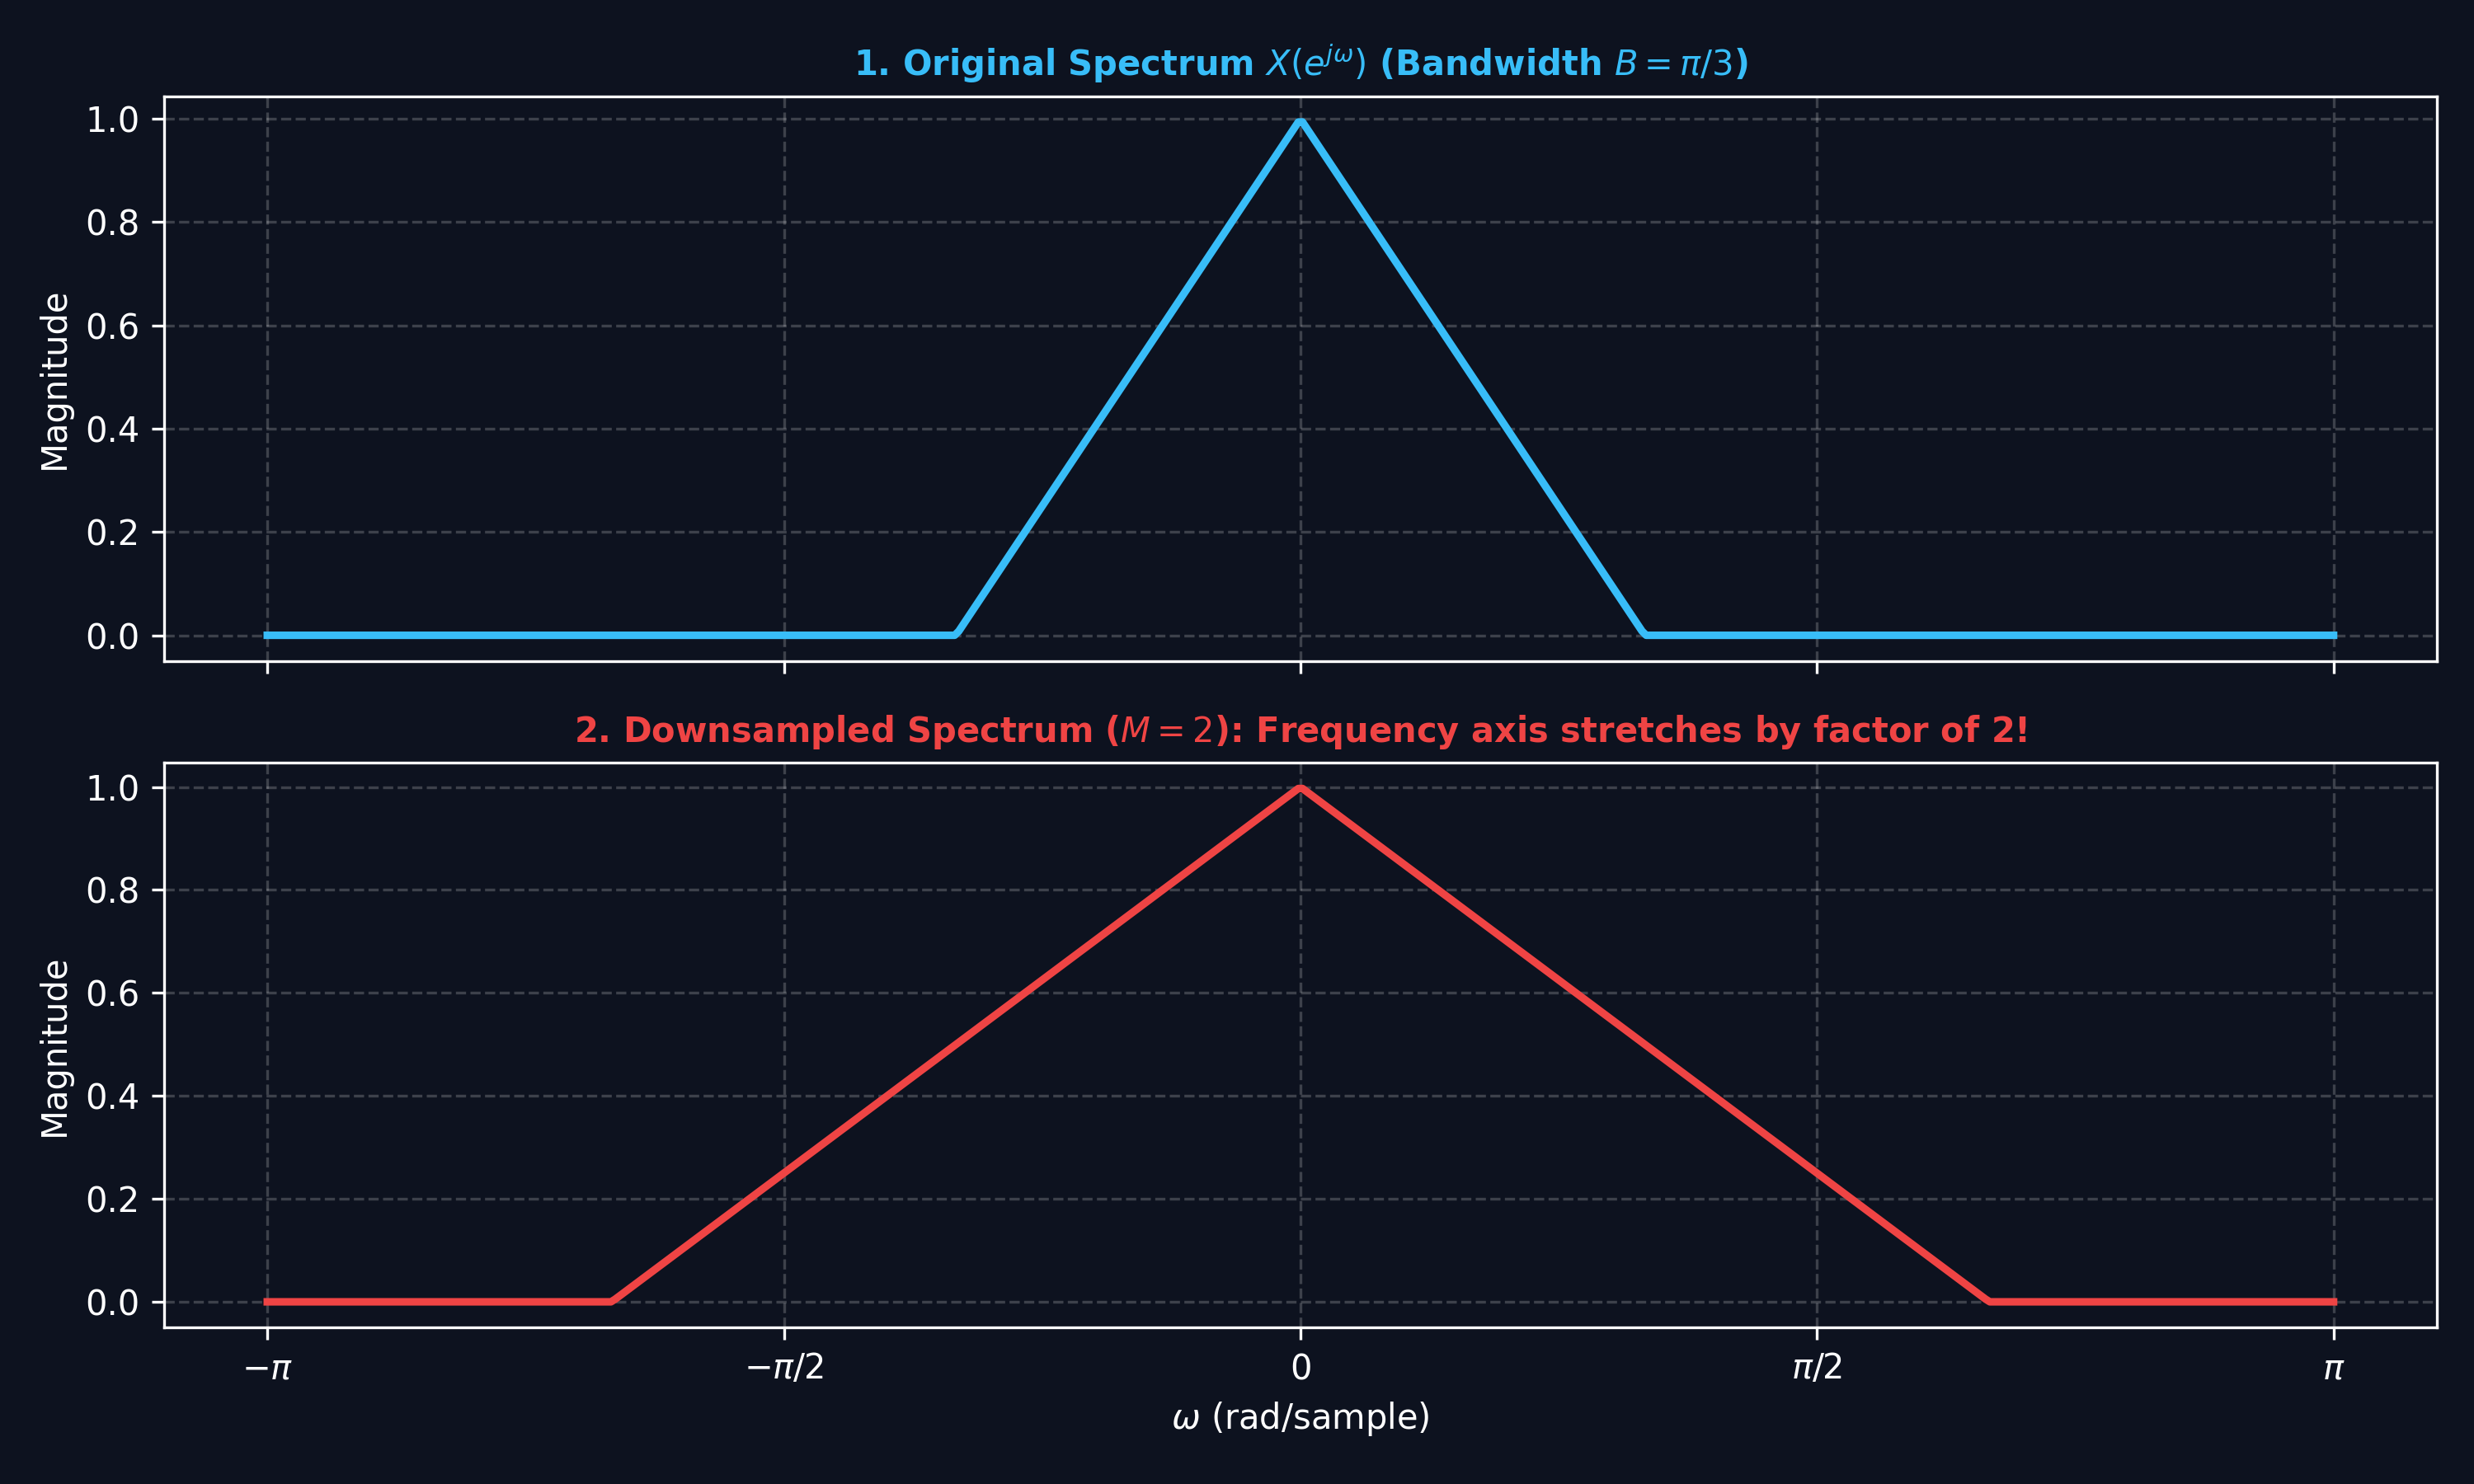
\includegraphics[width=0.85\textwidth]{images/downsampling_decimation_spectrum.png}
    \caption{Downsampling (Decimation) Frequency Spectrum: Frequency Axis Expansion and Anti-Aliasing Requirement.}
\end{figure}

\begin{figure}[H]
    \centering
    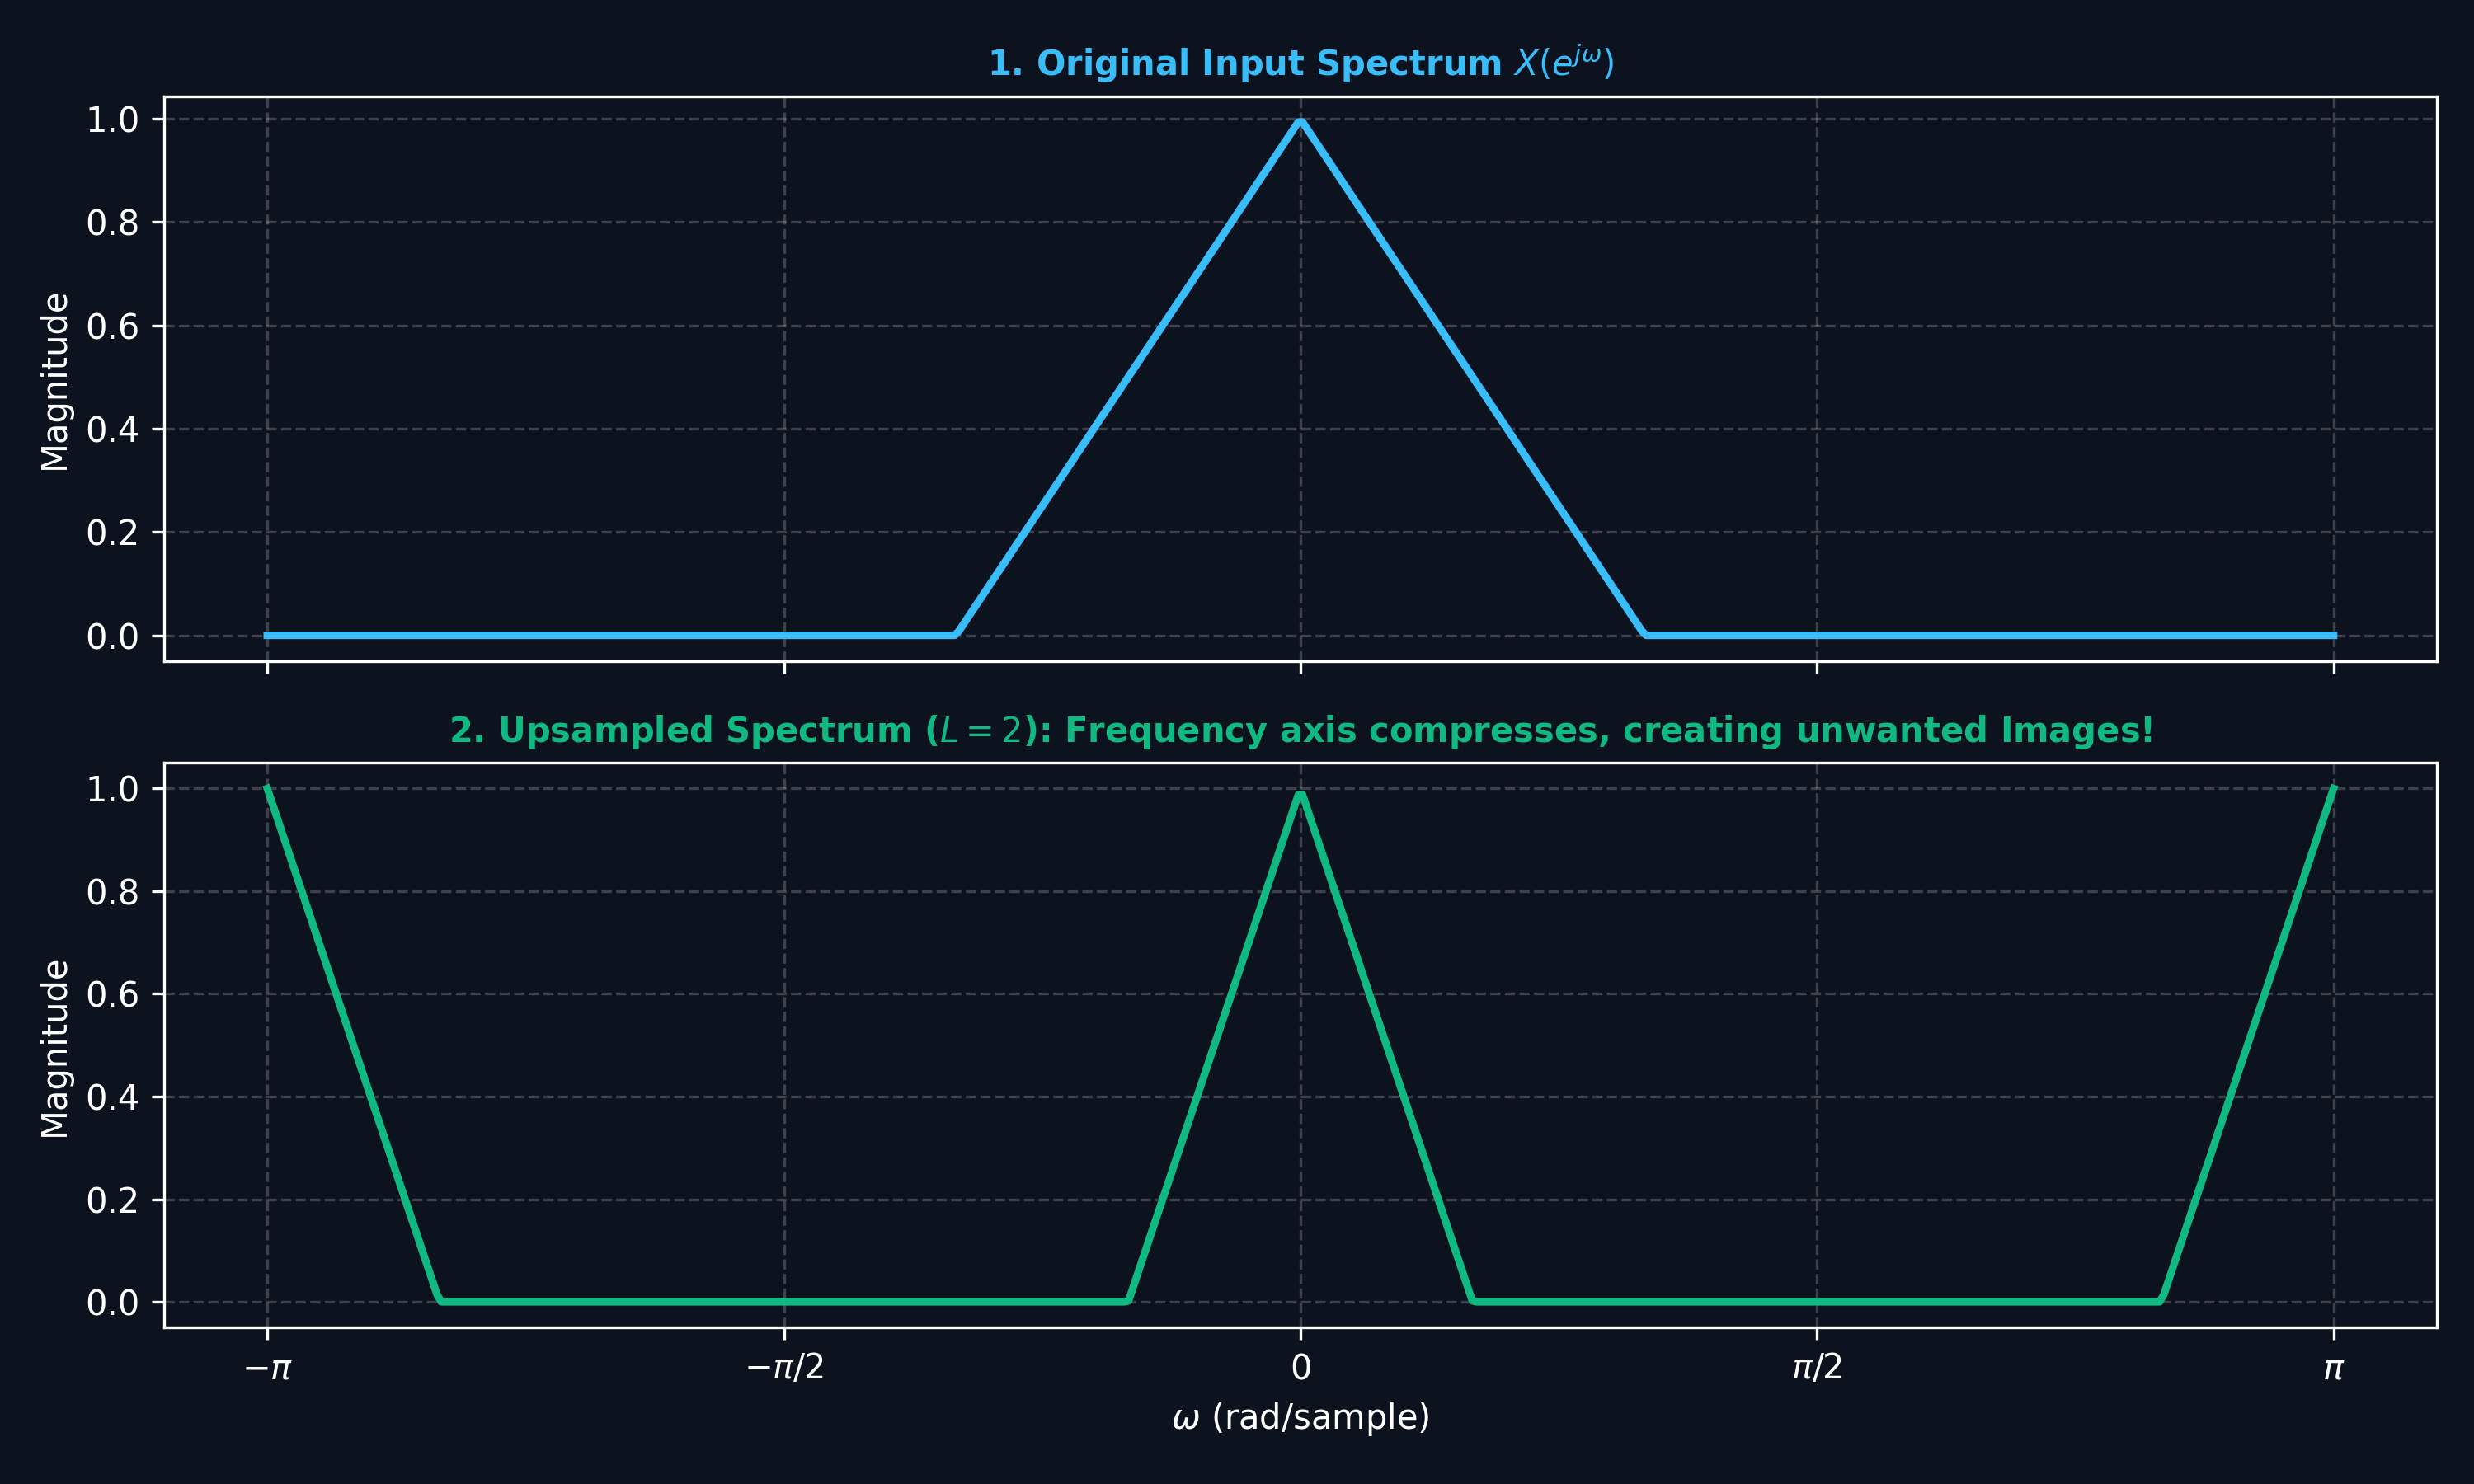
\includegraphics[width=0.85\textwidth]{images/upsampling_interpolation_spectrum.png}
    \caption{Upsampling (Interpolation) Spectrum: Zero-Insertion Spectral Compression and Anti-Imaging Filter.}
\end{figure}

\begin{figure}[H]
    \centering
    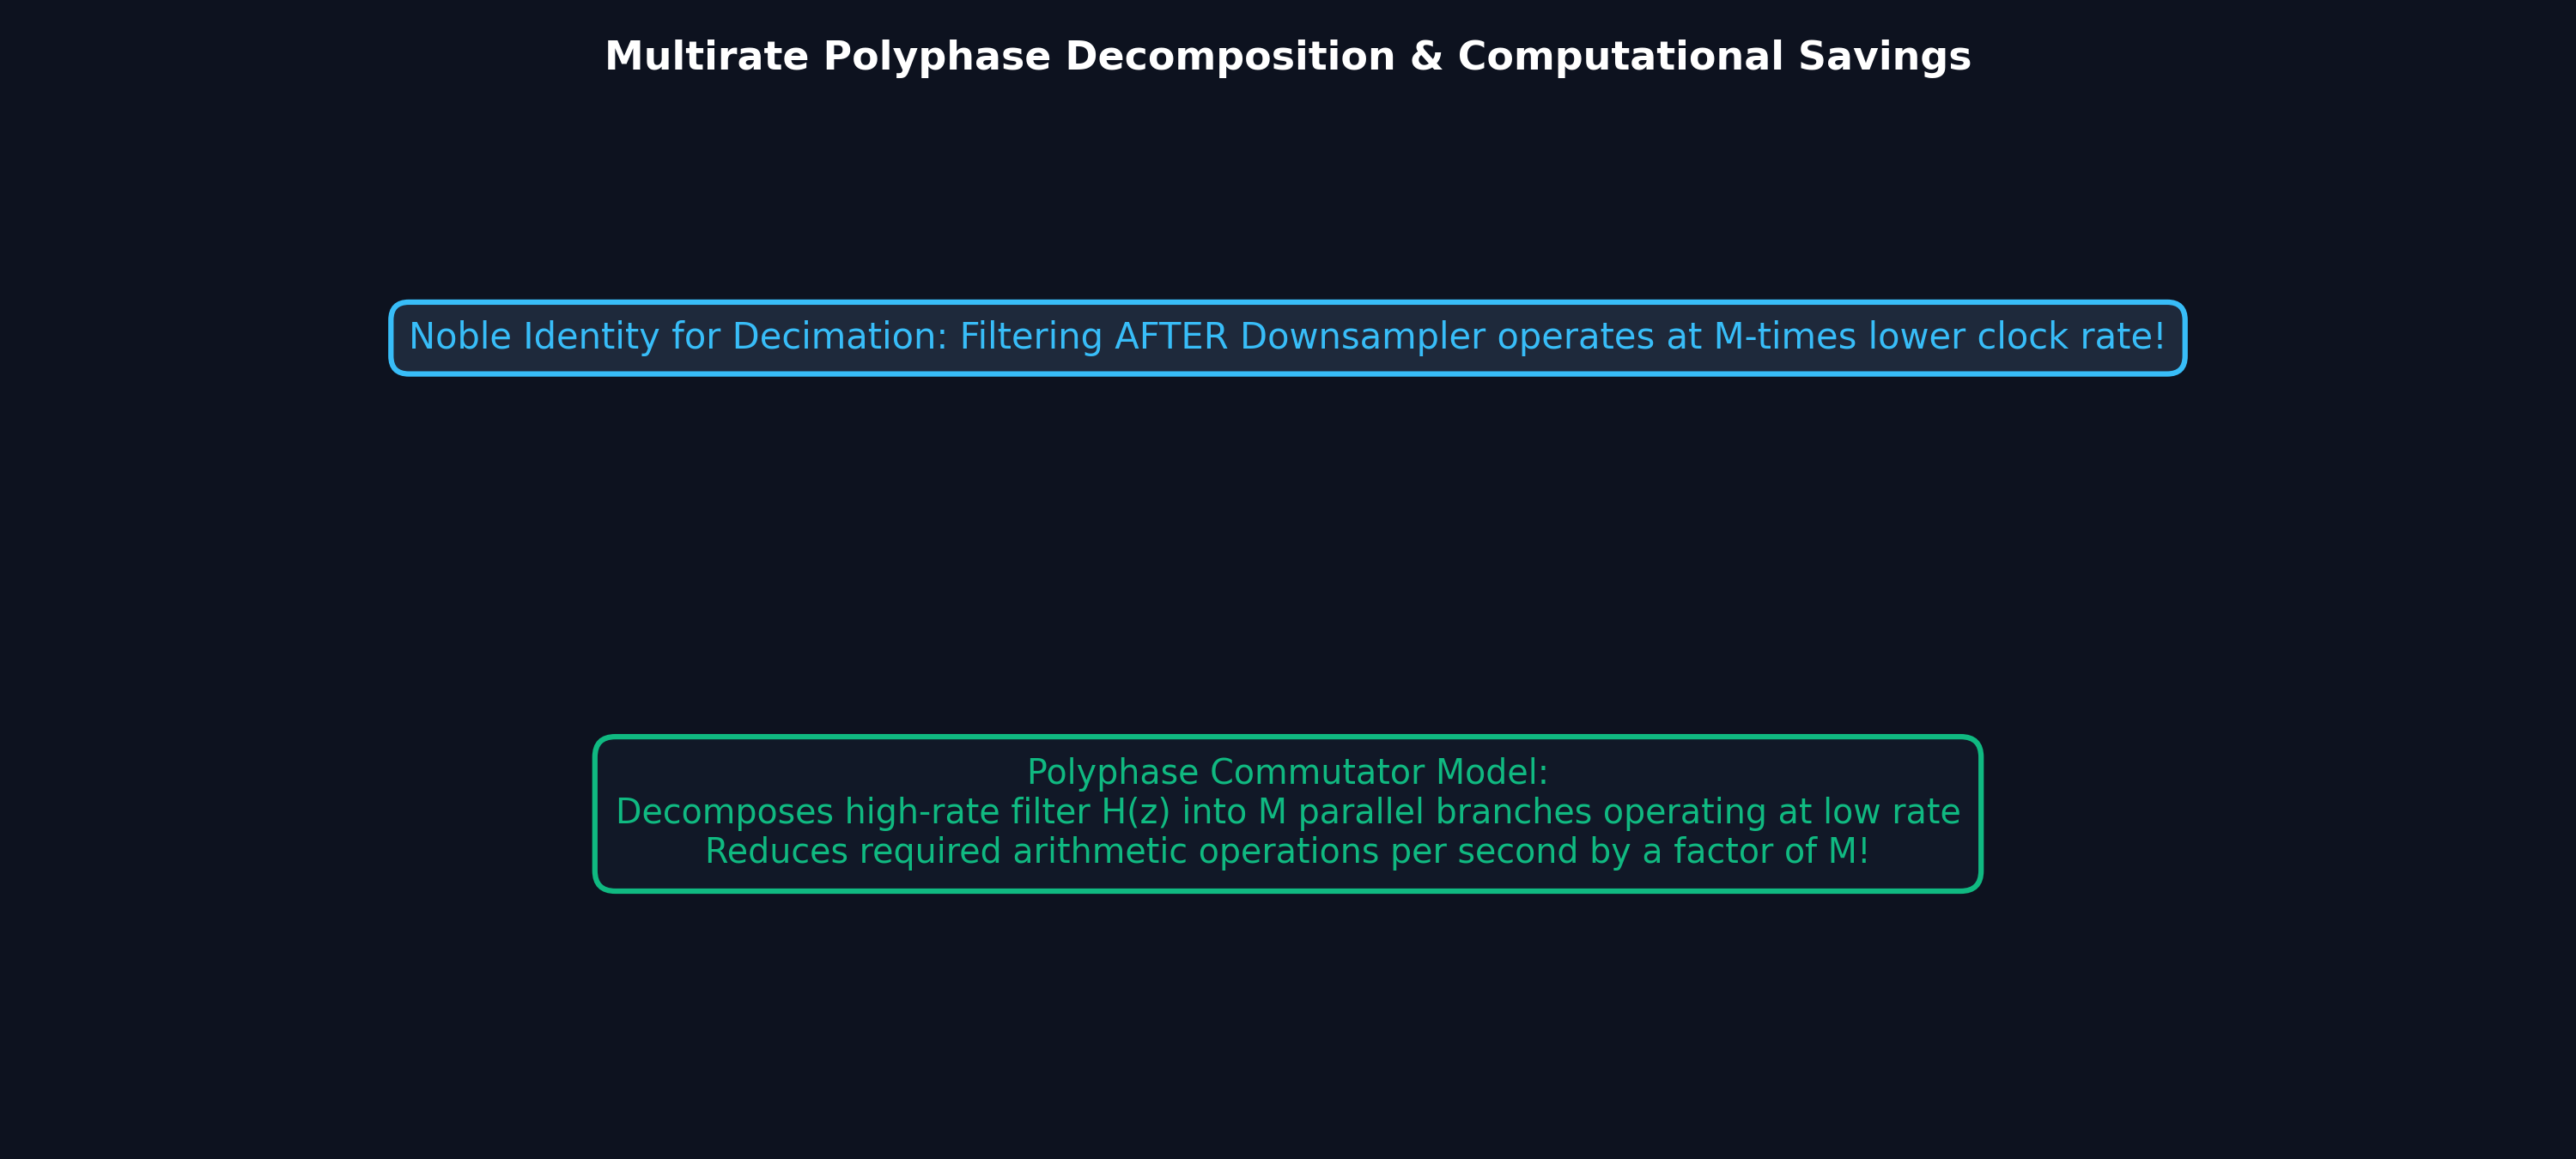
\includegraphics[width=0.85\textwidth]{images/polyphase_decomposition_noble.png}
    \caption{Multirate Polyphase Decomposition and Noble Identities for Efficient Low-Rate Implementation.}
\end{figure}


\subsection{Time-Domain Operation}
Downsampling (or sub-sampling) by an integer factor $M$ means we keep every $M$-th sample of the sequence and discard all the rest. The mathematical input-output relation is:
\begin{equation}
y[n] = x[Mn]
\end{equation}
For example, if $M=2$, the sequence $y[n]$ consists of $x[0], x[2], x[4], x[6], \dots$.

\subsection{Rigorous Frequency-Domain Derivation}
We want to find $Y(e^{j\omega})$, the Discrete-Time Fourier Transform (DTFT) of the downsampled signal $y[n]$, strictly in terms of the original spectrum $X(e^{j\omega})$.

\textbf{Step 1:} Define an intermediate sequence $v[n]$ that sets the discarded samples to zero, rather than removing them entirely.
\begin{equation}
v[n] = x[n] \cdot p[n]
\end{equation}
where $p[n]$ is a discrete-time impulse train:
\begin{equation}
p[n] = \begin{cases} 1, & n = kM \text{ for integer } k \\ 0, & \text{otherwise} \end{cases}
\end{equation}

\textbf{Step 2:} Express the periodic sequence $p[n]$ using its Discrete Fourier Series (DFS) representation:
\begin{equation}
p[n] = \frac{1}{M} \sum_{k=0}^{M-1} e^{j \frac{2\pi k}{M} n}
\end{equation}

\textbf{Step 3:} Substitute the DFS of $p[n]$ back into the equation for $v[n]$:
\begin{equation}
v[n] = \frac{1}{M} \sum_{k=0}^{M-1} x[n] e^{j \frac{2\pi k}{M} n}
\end{equation}

\textbf{Step 4:} Take the DTFT of $v[n]$. Multiplying by $e^{j \theta n}$ shifts the spectrum by $\theta$:
\begin{equation}
V(e^{j\omega}) = \sum_{n=-\infty}^{\infty} \left( \frac{1}{M} \sum_{k=0}^{M-1} x[n] e^{j \frac{2\pi k}{M} n} \right) e^{-j\omega n}
\end{equation}
\begin{equation}
V(e^{j\omega}) = \frac{1}{M} \sum_{k=0}^{M-1} X\left(e^{j\left(\omega - \frac{2\pi k}{M}\right)}\right)
\end{equation}

\textbf{Step 5:} Now, relate the final output $y[n]$ to the intermediate sequence $v[n]$. Notice that $v[n]$ has zeros everywhere except at integer multiples of $M$. At those multiples, $v[Mn] = x[Mn] = y[n]$.
Therefore, computing the DTFT of $y[n]$:
\begin{equation}
Y(e^{j\omega}) = \sum_{n=-\infty}^{\infty} v[Mn] e^{-j\omega n}
\end{equation}
Let us make a change of variables, setting $m = Mn$. Since $v[m]=0$ whenever $m$ is not a multiple of $M$, we can sum over all $m$:
\begin{equation}
Y(e^{j\omega}) = \sum_{m=-\infty}^{\infty} v[m] e^{-j\omega (m/M)} = V(e^{j\omega / M})
\end{equation}

\textbf{Step 6 (KEY RESULT):} Substitute the expression for $V(e^{j\omega})$ evaluated at $\omega / M$:
\begin{equation}
Y(e^{j\omega}) = \frac{1}{M} \sum_{k=0}^{M-1} X\left(e^{j\frac{\omega - 2\pi k}{M}}\right)
\end{equation}

\subsection{Aliasing and Anti-Aliasing Filter Design}
The final sum contains $M$ shifted copies of the original spectrum $X(e^{j\omega})$. Because we scale the frequency axis by $1/M$, the spectrum stretches outwards.
\begin{itemize}
    \item If the original spectrum $X(e^{j\omega})$ has energy at frequencies higher than $\pi/M$, the stretched, shifted copies will overlap with the baseband copy ($k=0$). This overlapping is \textbf{aliasing}.
    \item \textbf{Anti-Aliasing Filter:} To completely prevent this overlapping, we must ensure the signal is strictly band-limited to $|\omega| < \pi/M$ \emph{before} the downsampling step.
    \item We achieve this by applying a digital lowpass filter $H(e^{j\omega})$ with a cutoff frequency of $\omega_c = \pi/M$. The overall cascade of filtering followed by downsampling is formally called \textbf{decimation}.
\end{itemize}

\section{Upsampling by $L$ (Interpolation)}
\subsection{Time-Domain Operation}
Upsampling by an integer factor $L$ involves expanding the time base by inserting $L-1$ zeros between every pair of consecutive samples in the input sequence.
\begin{equation}
y[n] = \begin{cases} x[n/L], & n = kL \text{ for integer } k \\ 0, & \text{otherwise} \end{cases}
\end{equation}

\subsection{Rigorous Frequency-Domain Derivation}
Taking the DTFT of the upsampled sequence $y[n]$ directly:
\begin{equation}
Y(e^{j\omega}) = \sum_{n=-\infty}^{\infty} y[n] e^{-j\omega n}
\end{equation}
Since $y[n]$ is strictly non-zero only for indices $n = kL$:
\begin{equation}
Y(e^{j\omega}) = \sum_{k=-\infty}^{\infty} y[kL] e^{-j\omega (kL)} = \sum_{k=-\infty}^{\infty} x[k] e^{-j(\omega L)k}
\end{equation}
\textbf{KEY RESULT:}
\begin{equation}
Y(e^{j\omega}) = X(e^{j\omega L})
\end{equation}

\subsection{Imaging and Anti-Imaging Filter Design}
Because of the $\omega L$ term inside the argument, the original spectrum is compressed along the frequency axis by a factor of $L$.
\begin{itemize}
    \item Because all DTFT spectra are inherently $2\pi$-periodic, the compressed baseband spectrum repeats itself $L$ times within the $[-\pi, \pi]$ interval. These unwanted extra copies are called \textbf{spectral images}.
    \item \textbf{Anti-Imaging Filter:} To remove these zero-inserted artifacts and smoothly interpolate between the non-zero samples, we apply a lowpass filter with a cutoff frequency $\omega_c = \pi/L$.
    \item Since inserting $L-1$ zeros reduces the average energy per sample by a factor of $L$, this interpolation filter must have a DC gain of exactly $L$.
\end{itemize}

\section{Rational Rate Change ($L/M$)}
To change the sampling rate by a non-integer, rational factor like $L/M$, we cascade the upsampling and downsampling operations.
\begin{enumerate}
    \item \textbf{Upsample by $L$} (insert $L-1$ zeros).
    \item \textbf{Apply Interpolation Filter} (lowpass, cutoff $\pi/L$, gain $L$).
    \item \textbf{Apply Anti-Aliasing Filter} (lowpass, cutoff $\pi/M$, gain $1$).
    \item \textbf{Downsample by $M$} (keep every $M$-th sample).
\end{enumerate}
We combine the two filters into a single, highly efficient lowpass filter.
\begin{itemize}
    \item The combined filter's cutoff frequency is $\omega_c = \min(\pi/L, \pi/M)$.
    \item The combined filter must preserve the gain required by the interpolation step, so its gain remains $L$.
\end{itemize}
\textbf{Crucial note:} Always upsample first, filter, and then downsample. Downsampling first would cause permanent aliasing.

\section{Noble Identities}
The \textbf{Noble Identities} are fundamental theorems that allow us to commute filters and multirate blocks.

\subsection{First Noble Identity: Decimation Identity}
\textbf{Statement:} Filtering with a transfer function $H(z)$ followed by downsampling $\downarrow M$ is exactly equivalent to downsampling $\downarrow M$ first, followed by filtering with $H(z^M)$.

\textbf{Proof:}
Consider the right side block diagram: an input $x[n]$ is downsampled by $M$ to produce $w[n]$, which is then filtered by $H(z)$ to produce $y[n]$.
\begin{equation}
W(z) = \frac{1}{M} \sum_{k=0}^{M-1} X(z^{1/M} W_M^k) \quad \text{where } W_M = e^{-j2\pi/M}
\end{equation}
\begin{equation}
Y(z) = W(z)H(z) = H(z) \left[ \frac{1}{M} \sum_{k=0}^{M-1} X(z^{1/M} W_M^k) \right]
\end{equation}

Now consider the left side: $x[n]$ is passed through a filter $H(z^M)$ to produce $v[n]$, which is then downsampled by $M$.
\begin{equation}
V(z) = X(z)H(z^M)
\end{equation}
After downsampling $v[n]$ by $M$, we get $Y'(z)$:
\begin{equation}
Y'(z) = \frac{1}{M} \sum_{k=0}^{M-1} \left[ X(z^{1/M} W_M^k) \cdot H((z^{1/M} W_M^k)^M) \right]
\end{equation}
Since $(z^{1/M} W_M^k)^M = z \cdot e^{-j2\pi k} = z$, the filter argument simplifies to $z$:
\begin{equation}
Y'(z) = H(z) \left[ \frac{1}{M} \sum_{k=0}^{M-1} X(z^{1/M} W_M^k) \right]
\end{equation}
Thus $Y(z) = Y'(z)$, rigorously proving the identity.

\subsection{Second Noble Identity: Interpolation Identity}
\textbf{Statement:} Upsampling $\uparrow L$ followed by filtering with $H(z^L)$ is exactly equivalent to filtering with $H(z)$ followed by upsampling $\uparrow L$.

\textbf{Proof:}
Left side: input $x[n]$ passes through $H(z)$ to produce $v[n]$, then is upsampled by $L$.
\begin{equation}
V(z) = H(z)X(z) \implies Y(z) = V(z^L) = H(z^L)X(z^L)
\end{equation}

Right side: input $x[n]$ is upsampled by $L$ to produce $w[n]$, then passes through $H(z^L)$.
\begin{equation}
W(z) = X(z^L) \implies Y'(z) = H(z^L)W(z) = H(z^L)X(z^L)
\end{equation}
Since $Y(z) = Y'(z)$, the interpolation identity is proved.

\section{Polyphase Decomposition}
Polyphase structures are the key to realizing multirate filters efficiently in practical hardware.

\subsection{Detailed Mathematical Formulation}
Any transfer function $H(z) = \sum h[n]z^{-n}$ can be deterministically split into $M$ parallel sub-filters, known as polyphase components.
\begin{equation}
H(z) = \sum_{k=0}^{M-1} z^{-k} E_k(z^M)
\end{equation}
where the $k$-th polyphase component is defined as:
\begin{equation}
E_k(z) = \sum_{n=-\infty}^{\infty} h[Mn+k]z^{-n}
\end{equation}

\subsection{Why is this massively useful for Decimation ($M:1$)?}
In a direct implementation of a decimation filter, we compute the convolution to calculate every single output sample, and then the downsampler throws away $M-1$ out of every $M$ samples. This wastes huge amounts of arithmetic logic.

Using polyphase decomposition, we write $H(z) = E_0(z^M) + z^{-1}E_1(z^M) + \dots + z^{-(M-1)}E_{M-1}(z^M)$. By applying the \textbf{First Noble Identity}, we can move the downsampler $\downarrow M$ to sit \emph{before} the filters $E_k(z)$. This means we downsample the input data stream \emph{first}, and then run the sub-filters $E_k(z)$ at the much \emph{lower} sampling rate, reducing the arithmetic workload by a factor of $M$.

\subsection{The Commutator Model}
Instead of explicitly writing delay chains and individual downsamplers, engineers model the input routing as a counter-clockwise rotating switch (a commutator). This switch distributes the incoming high-rate input samples sequentially to the $M$ parallel polyphase filters, which operate continuously at the lower rate.

\section{Summary of Key Formulas}
\begin{table}[H]
\centering
\caption{Key Multirate Formulas}
\begin{tabular}{l l l}
\toprule
\textbf{Operation} & \textbf{Time Domain} & \textbf{Frequency/Z Domain} \\
\midrule
Downsample ($M$) & $y[n] = x[Mn]$ & $Y(z) = \frac{1}{M}\sum_{k=0}^{M-1} X(z^{1/M} e^{-j2\pi k/M})$ \\
Upsample ($L$) & $y[n] = x[n/L]$ for $n=kL$, else 0 & $Y(z) = X(z^L)$ \\
Noble ID (Dec) & $H(z^M)$ then $\downarrow M$ & equals $\downarrow M$ then $H(z)$ \\
Noble ID (Int) & $\uparrow L$ then $H(z^L)$ & equals $H(z)$ then $\uparrow L$ \\
Polyphase & $E_k(z) = \sum h[Mn+k]z^{-n}$ & $H(z) = \sum_{k=0}^{M-1} z^{-k} E_k(z^M)$ \\
\bottomrule
\end{tabular}
\end{table}

\section{Checkpoint Questions \& Detailed Worked Examples}
\begin{enumerate}
    \item \textbf{Downsampling Spectra and Bandwidth Tracking:} 
    Suppose a discrete-time signal $x[n]$ has a spectrum $X(e^{j\omega})$ that is non-zero only for $|\omega| \le \pi/4$. We downsample this signal by $M=3$. Will there be aliasing? What is the absolute bandwidth of the new downsampled signal $y[n]$? \\
    \textit{Answer:} The fundamental condition to avoid aliasing is that the original signal must be bandlimited to $\pi/M = \pi/3 \approx 1.047 \text{ rad/s}$. The signal is bandlimited to $\pi/4 \approx 0.785 \text{ rad/s}$. Because $\pi/4 < \pi/3$, the shifted copies will not overlap with the baseband, meaning \textbf{there is absolutely no aliasing}. Downsampling stretches the spectrum by a factor of 3. The new bandwidth is $3 \times (\pi/4) = 3\pi/4$.
    
    \item \textbf{Extracting Polyphase Components:} 
    Given $h[n] = \{1, 2, 3, 4, 5, 6, 7\}$ (with origin at $h[0]=1$). Extract the z-domain expressions for the polyphase components $E_0(z)$ and $E_1(z)$ when $M=2$. \\
    \textit{Answer:} For $M=2$, we split $h[n]$ into even and odd indices. \\
    \textbf{Finding $E_0(z)$:} Takes even samples $\{h[0], h[2], h[4], h[6]\} = \{1, 3, 5, 7\}$. \\
    $E_0(z) = 1 + 3z^{-1} + 5z^{-2} + 7z^{-3}$. \\
    \textbf{Finding $E_1(z)$:} Takes odd samples $\{h[1], h[3], h[5]\} = \{2, 4, 6\}$. \\
    $E_1(z) = 2 + 4z^{-1} + 6z^{-2}$.
    
    \item \textbf{Rational Rate Conversion Architecture Design:} 
    Convert $44.1\text{ kHz}$ to $48\text{ kHz}$. What are $L$ and $M$? What is the exact digital cutoff frequency? \\
    \textit{Answer:} The ratio is $48000 / 44100 = 160 / 147$. We upsample by $L = 160$ and downsample by $M = 147$. The intermediate filter must prevent both imaging (cutoff $\pi/160$) and aliasing (cutoff $\pi/147$). The combined filter uses the lower cutoff: $\omega_c = \min(\pi/160, \pi/147) = \pi/160 \text{ rad/sample}$.
    
    \item \textbf{The Noble Identity in Practice:}
    A system upsamples a signal by $L=4$, and then applies a filter $H_{old}(z) = 1 - z^{-8} + 0.5z^{-12}$. Draw a computationally cheaper equivalent system. \\
    \textit{Answer:} The original system is $x[n] \to \uparrow 4 \to H_{old}(z) \to y[n]$. Notice $H_{old}(z)$ is a function of $z^4$, so we can write it as $H_{new}(z^4)$ where $H_{new}(z) = 1 - z^{-2} + 0.5z^{-3}$. By the Second Noble Identity, upsampling by $4$ then filtering with $H_{new}(z^4)$ equals filtering with $H_{new}(z)$ then upsampling by $4$. The cheaper system is $x[n] \to H_{new}(z) \to \uparrow 4 \to y[n]$.
\end{enumerate}

\end{document}
